% Options for packages loaded elsewhere
% Options for packages loaded elsewhere
\PassOptionsToPackage{unicode}{hyperref}
\PassOptionsToPackage{hyphens}{url}
\PassOptionsToPackage{dvipsnames,svgnames,x11names}{xcolor}
%
\documentclass[
  english,
  10pt,
  letterpaper,
  DIV=11,
  numbers=noendperiod]{scrartcl}
\usepackage{xcolor}
\usepackage[margin=1in]{geometry}
\usepackage{amsmath,amssymb}
\setcounter{secnumdepth}{5}
\usepackage{iftex}
\ifPDFTeX
  \usepackage[T1]{fontenc}
  \usepackage[utf8]{inputenc}
  \usepackage{textcomp} % provide euro and other symbols
\else % if luatex or xetex
  \usepackage{unicode-math} % this also loads fontspec
  \defaultfontfeatures{Scale=MatchLowercase}
  \defaultfontfeatures[\rmfamily]{Ligatures=TeX,Scale=1}
\fi
\usepackage{lmodern}
\ifPDFTeX\else
  % xetex/luatex font selection
\fi
% Use upquote if available, for straight quotes in verbatim environments
\IfFileExists{upquote.sty}{\usepackage{upquote}}{}
\IfFileExists{microtype.sty}{% use microtype if available
  \usepackage[]{microtype}
  \UseMicrotypeSet[protrusion]{basicmath} % disable protrusion for tt fonts
}{}
\makeatletter
\@ifundefined{KOMAClassName}{% if non-KOMA class
  \IfFileExists{parskip.sty}{%
    \usepackage{parskip}
  }{% else
    \setlength{\parindent}{0pt}
    \setlength{\parskip}{6pt plus 2pt minus 1pt}}
}{% if KOMA class
  \KOMAoptions{parskip=half}}
\makeatother
% Make \paragraph and \subparagraph free-standing
\makeatletter
\ifx\paragraph\undefined\else
  \let\oldparagraph\paragraph
  \renewcommand{\paragraph}{
    \@ifstar
      \xxxParagraphStar
      \xxxParagraphNoStar
  }
  \newcommand{\xxxParagraphStar}[1]{\oldparagraph*{#1}\mbox{}}
  \newcommand{\xxxParagraphNoStar}[1]{\oldparagraph{#1}\mbox{}}
\fi
\ifx\subparagraph\undefined\else
  \let\oldsubparagraph\subparagraph
  \renewcommand{\subparagraph}{
    \@ifstar
      \xxxSubParagraphStar
      \xxxSubParagraphNoStar
  }
  \newcommand{\xxxSubParagraphStar}[1]{\oldsubparagraph*{#1}\mbox{}}
  \newcommand{\xxxSubParagraphNoStar}[1]{\oldsubparagraph{#1}\mbox{}}
\fi
\makeatother


\usepackage{longtable,booktabs,array}
\newcounter{none} % for unnumbered tables
\usepackage{calc} % for calculating minipage widths
% Correct order of tables after \paragraph or \subparagraph
\usepackage{etoolbox}
\makeatletter
\patchcmd\longtable{\par}{\if@noskipsec\mbox{}\fi\par}{}{}
\makeatother
% Allow footnotes in longtable head/foot
\IfFileExists{footnotehyper.sty}{\usepackage{footnotehyper}}{\usepackage{footnote}}
\makesavenoteenv{longtable}
\usepackage{graphicx}
\makeatletter
\newsavebox\pandoc@box
\newcommand*\pandocbounded[1]{% scales image to fit in text height/width
  \sbox\pandoc@box{#1}%
  \Gscale@div\@tempa{\textheight}{\dimexpr\ht\pandoc@box+\dp\pandoc@box\relax}%
  \Gscale@div\@tempb{\linewidth}{\wd\pandoc@box}%
  \ifdim\@tempb\p@<\@tempa\p@\let\@tempa\@tempb\fi% select the smaller of both
  \ifdim\@tempa\p@<\p@\scalebox{\@tempa}{\usebox\pandoc@box}%
  \else\usebox{\pandoc@box}%
  \fi%
}
% Set default figure placement to htbp
\def\fps@figure{htbp}
\makeatother


% definitions for citeproc citations
\NewDocumentCommand\citeproctext{}{}
\NewDocumentCommand\citeproc{mm}{%
  \begingroup\def\citeproctext{#2}\cite{#1}\endgroup}
\makeatletter
 % allow citations to break across lines
 \let\@cite@ofmt\@firstofone
 % avoid brackets around text for \cite:
 \def\@biblabel#1{}
 \def\@cite#1#2{{#1\if@tempswa , #2\fi}}
\makeatother
\newlength{\cslhangindent}
\setlength{\cslhangindent}{1.5em}
\newlength{\csllabelwidth}
\setlength{\csllabelwidth}{3em}
\newenvironment{CSLReferences}[2] % #1 hanging-indent, #2 entry-spacing
 {\begin{list}{}{%
  \setlength{\itemindent}{0pt}
  \setlength{\leftmargin}{0pt}
  \setlength{\parsep}{0pt}
  % turn on hanging indent if param 1 is 1
  \ifodd #1
   \setlength{\leftmargin}{\cslhangindent}
   \setlength{\itemindent}{-1\cslhangindent}
  \fi
  % set entry spacing
  \setlength{\itemsep}{#2\baselineskip}}}
 {\end{list}}
\usepackage{calc}
\newcommand{\CSLBlock}[1]{\hfill\break\parbox[t]{\linewidth}{\strut\ignorespaces#1\strut}}
\newcommand{\CSLLeftMargin}[1]{\parbox[t]{\csllabelwidth}{\strut#1\strut}}
\newcommand{\CSLRightInline}[1]{\parbox[t]{\linewidth - \csllabelwidth}{\strut#1\strut}}
\newcommand{\CSLIndent}[1]{\hspace{\cslhangindent}#1}

\ifLuaTeX
\usepackage[bidi=basic,shorthands=off]{babel}
\else
\usepackage[bidi=default,shorthands=off]{babel}
\fi
\ifLuaTeX
  \usepackage{selnolig} % disable illegal ligatures
\fi


\setlength{\emergencystretch}{3em} % prevent overfull lines

\providecommand{\tightlist}{%
  \setlength{\itemsep}{0pt}\setlength{\parskip}{0pt}}



 


\KOMAoption{captions}{tableheading}
\makeatletter
\@ifpackageloaded{caption}{}{\usepackage{caption}}
\AtBeginDocument{%
\ifdefined\contentsname
  \renewcommand*\contentsname{Table of contents}
\else
  \newcommand\contentsname{Table of contents}
\fi
\ifdefined\listfigurename
  \renewcommand*\listfigurename{List of Figures}
\else
  \newcommand\listfigurename{List of Figures}
\fi
\ifdefined\listtablename
  \renewcommand*\listtablename{List of Tables}
\else
  \newcommand\listtablename{List of Tables}
\fi
\ifdefined\figurename
  \renewcommand*\figurename{Figure}
\else
  \newcommand\figurename{Figure}
\fi
\ifdefined\tablename
  \renewcommand*\tablename{Table}
\else
  \newcommand\tablename{Table}
\fi
}
\@ifpackageloaded{float}{}{\usepackage{float}}
\floatstyle{ruled}
\@ifundefined{c@chapter}{\newfloat{codelisting}{h}{lop}}{\newfloat{codelisting}{h}{lop}[chapter]}
\floatname{codelisting}{Listing}
\newcommand*\listoflistings{\listof{codelisting}{List of Listings}}
\makeatother
\makeatletter
\makeatother
\makeatletter
\@ifpackageloaded{caption}{}{\usepackage{caption}}
\@ifpackageloaded{subcaption}{}{\usepackage{subcaption}}
\makeatother
\usepackage{bookmark}
\IfFileExists{xurl.sty}{\usepackage{xurl}}{} % add URL line breaks if available
\urlstyle{same}
% fallback for those not using the hyperref driver hyperxmp:
\makeatletter
\@ifundefined{xmpquote}{\newcommand{\xmpquote}[1]{#1}}{}
\makeatother
\hypersetup{
  pdftitle={Exact Term Structure of Stochastic Correlation},
  pdfauthor={Complex--Itô Random-Walk Research Project},
  pdflang={en},
  pdfkeywords={\xmpquote{stochastic
correlation}, \xmpquote{time-inhomogeneous
diffusion}, \xmpquote{Feynman-Kac}, \xmpquote{boundary
crossing}, \xmpquote{term structure}, \xmpquote{operational time}},
  colorlinks=true,
  linkcolor={blue},
  filecolor={Maroon},
  citecolor={Blue},
  urlcolor={Blue},
  pdfcreator={LaTeX via pandoc}}


\title{Exact Term Structure of Stochastic Correlation}
\usepackage{etoolbox}
\makeatletter
\providecommand{\subtitle}[1]{% add subtitle to \maketitle
  \apptocmd{\@title}{\par {\large #1 \par}}{}{}
}
\makeatother
\subtitle{Static Inheritance, the Proportional-Drift Class, and a
Feynman--Kac Pitfall for Non-Autonomous Drivers}
\author{Complex--Itô Random-Walk Research Project}
\date{August 21, 2026}
\begin{document}
\maketitle
\begin{abstract}
We extend an exact-law framework for stochastic correlation
\(\rho_t=f(X_t)=X_t/\sqrt{X_t^2+c^2}\), previously developed under
constant driver coefficients \((\mu,\sigma)\), to deterministic
coefficient curves \(\mu(t),\sigma(t)\). Three results structure the
extension. First, a static-inheritance theorem: every law of \(\rho\)
that depends on finitely many marginals or transitions is the
constant-coefficient formula with \(m(t)=x_0+\int\mu\) and
\(v(t)=\int\sigma^2\), yielding --- among objects not published in any
audited competitor --- an exact closed-form quantile term structure
\(q_\alpha(t)\), exact forward-start digitals, and a two-parameter
bootstrap of \((c,\lambda^{\mathbb Q})\) from correlation-digital
quotes. Second, a classification theorem: on the proportional-drift
class \(\mu(t)=\lambda\sigma^2(t)\) the Dambis--Dubins--Schwarz theorem
collapses every reflection-principle barrier law to operational time
\(u=v(T)\), with barrier prices depending on the volatility curve only
through integrated variance (a parsimony corollary); off this class the
known catalog contains no closed forms. Third, a negative structural
result with practical consequence: the backward Feynman--Kac equation
\(\partial_tu=\mathcal L_tu+q(x)u\) --- exact for constant coefficients
and the standard computational workhorse --- is \emph{violated} by
occupation functionals when coefficients depend on calendar time; we
give a drift-only counterexample and show that the correct primitive is
the forward Fokker--Planck equation with potential, which we implement
by Crank--Nicolson stepping and verify against closed forms,
second-order convergence, and Monte Carlo within four standard errors.
The failure is invisible to marginal-moment validation and appears only
under path-functional law checks.
\end{abstract}

\renewcommand*\contentsname{Table of contents}
{
\setcounter{tocdepth}{2}
\tableofcontents
}

\textbf{Mathematics Subject Classification (2020):} 60H10, 60J60, 60J65,
91G20, 91G60.

\textbf{JEL classification:} C02, C63, G12, G13.

\section{Introduction}\label{sec-introduction}

Bounded stochastic-correlation models stop, almost uniformly, at their
stationary density. The hyperbolic-OU family of Teng et al. (2016)
calibrates a histogram; simulation handles the rest. The bounded-factor
framework of the companion papers broke that ceiling for constant driver
coefficients: because \(\rho_t=X_t/\sqrt{X_t^2+c^2}\) is a monotone
conjugacy of a Gaussian factor, transition densities,
reflection-principle first-passage laws, corridor occupation laws, and
--- through Dambis--Dubins--Schwarz (DDS) --- the full clock law
underlying spread/basket pricing are available in closed form or as
one-dimensional deterministic quadratures.

This paper asks the natural robustness question: \textbf{which of these
laws survive when the driver has deterministic coefficient curves}
\(dX_t=\mu(t)\,dt+\sigma(t)\,dW_t\)? The question matters because any
term-structure calibration requires time dependence, and because the
answer is not uniform: some layers survive exactly, one survives on a
precisely characterizable class, and one standard tool fails silently.

The contributions are threefold.

\begin{enumerate}
\def\labelenumi{\arabic{enumi}.}
\tightlist
\item
  \textbf{Static inheritance} (Section~\ref{sec-static}): all
  finite-dimensional laws are the constant-coefficient formulas with
  \((m(t),v(t))\). This includes the exact quantile term structure
  \(q_\alpha(t)=f(m(t)+\sqrt{v(t)}\,
  \Phi^{-1}(\alpha))\), forward-start digitals, discrete range accruals,
  and a bootstrap of \((c,\lambda^{\mathbb Q})\) from digital quotes.
\item
  \textbf{The proportional-drift class}
  (Section~\ref{sec-proportional}): \(\mu(t)=\lambda\sigma^2(t)\) is
  exactly the class on which the reflection-principle toolkit survives,
  via DDS collapse to operational time; barrier laws depend on
  \(\sigma(\cdot)\) only through \(v(T)\).
\item
  \textbf{A Feynman--Kac pitfall} (Section~\ref{sec-pitfall}): the
  backward equation fails for occupation functionals off constant
  coefficients. The failure is invisible to marginal checks; we exhibit
  it numerically, diagnose it, and implement the correct forward
  equation.
\end{enumerate}

Throughout, ``exact'' means closed form up to elementary special
functions or one-dimensional quadrature; Monte Carlo is used only as
benchmark. All claims carry unit tests
(\texttt{tests/test\_phase7\_term\_structure.py}, 21 tests) and a
reproducible notebook (seed 20260821). The web-audited novelty boundary
is recorded in \texttt{PHASE\_7\_LITERATURE\_REVIEW.md}: closed-form
boundary crossing exists only for linear boundaries and isolated special
families (Durbin 1992; Pötzelberger and Wang 2001; Kahalé 2008), and no
audited competitor publishes exact correlation term structures.

\section{Setup}\label{sec-setup}

Let

\[
dX_t=\mu(t)\,dt+\sigma(t)\,dW_t,\qquad X_0=x_0,
\]

with \(\mu,\sigma\) deterministic, locally integrable /
square-integrable, and define the mean and variance curves

\[
m(t)=x_0+\int_0^t\mu(s)\,ds,\qquad v(t)=\int_0^t\sigma(s)^2\,ds .
\]

The correlation coordinate is \(\rho_t=f(X_t)\) with
\(f(x)=x/\sqrt{x^2+c^2}\), \(c>0\); its inverse in the conjugate
coordinate is \(x(\rho)=c\,\rho/\sqrt{1-\rho^2}\) with Jacobian
\(|dx/d\rho|=c(1-\rho^2)^{-3/2}\).

\section{Static inheritance}\label{sec-static}

\textbf{Theorem (static inheritance).} \emph{For every \(t\),
\(X_t\sim N(m(t),v(t))\); for every \(s<t\),
\(X_t\mid X_s\sim N(X_s+M_{st},V_{st})\) with \(M_{st}=\int_s^t\mu\),
\(V_{st}=\int_s^t\sigma^2\). Consequently every price or law depending
on finitely many marginals/transitions of \(\rho\) equals its
constant-coefficient counterpart with \((m(t_i),v(t_i))\) substituted.}

Immediate corollaries, each verified against Phase-6 anchors at
\(10^{-13}\) in the constant limit and against exact-skeleton Monte
Carlo within \textasciitilde1 SE:

\begin{itemize}
\tightlist
\item
  \textbf{Transition density}
  \[p_t(\rho\mid\rho_s)=\frac{c}{(1-\rho^2)^{3/2}}\,
  \varphi\!\left(\frac{x(\rho)-x(\rho_s)-M_{st}}{\sqrt{V_{st}}}\right).\]
\item
  \textbf{Expiry digitals}:
  \(e^{-rT}\Phi((m(T)-x(\rho^*))/\sqrt{v(T)})\).
\item
  \textbf{Forward-start digitals}: conditional on \(\rho_s\),
  \[E[1\{\rho_T\ge\rho^*\}\mid\rho_s]
  =\Phi\!\left(\frac{x(\rho_s)+M_{st}-x(\rho^*)}{\sqrt{V_{st}}}\right),\]
  and the tower property over the start marginal closes back to the
  unconditional formula (verified to \(10^{-10}\) by Gauss--Hermite).
\item
  \textbf{Discrete range accruals}: sum of per-date band probabilities.
\item
  \textbf{Quantile term structure}:
  \[q_\alpha(t)=f\big(m(t)+\sqrt{v(t)}\,\Phi^{-1}(\alpha)\big),\]
  continuous and strictly increasing in \(\alpha\); MC-checked at
  fifteen \((\alpha,t)\) points to 0.0033 maximum error
  (Figure~\ref{fig-quantiles}).
\end{itemize}

\begin{figure}[tbp]

\centering{

\pandocbounded{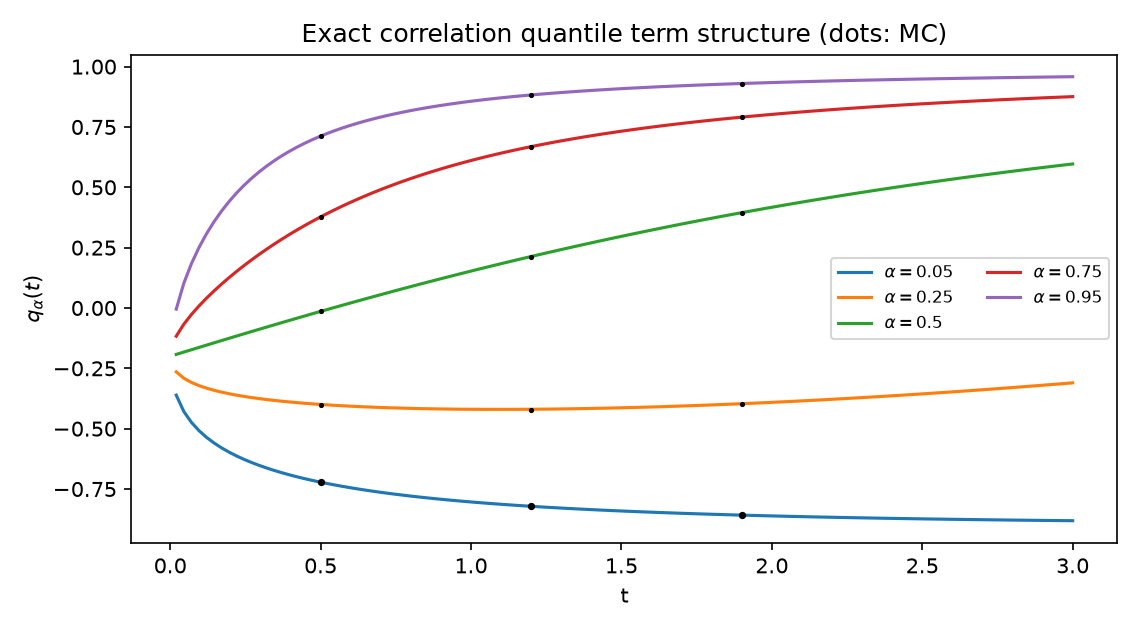
\includegraphics[keepaspectratio]{figures/phase7_quantile_term_structure.png}}

}

\caption{\label{fig-quantiles}Exact correlation quantile term structure
under a humped volatility curve; dots are Monte Carlo empirical
quantiles.}

\end{figure}%

\textbf{Bootstrap.} Correlation-digital quotes
\((T_j,\rho_j^*,\text{price}_j)\) identify \((c,\lambda^{\mathbb Q})\)
under the model of Section~\ref{sec-proportional} by two-parameter least
squares. On synthetic markets generated at \((c,\lambda)=(1.25,0.30)\)
recovery is exact to \(10^{-8}\) and the SSE landscape is single-funnel
(Figure~\ref{fig-bootstrap}). Identification here is \emph{not}
contradicted by the scale observational equivalence theorem of the
estimation paper: the volatility curve \(\sigma(\cdot)\) is exogenous,
which breaks the scaling degeneracy through the time ruler.

\begin{figure}[tbp]

\centering{

\pandocbounded{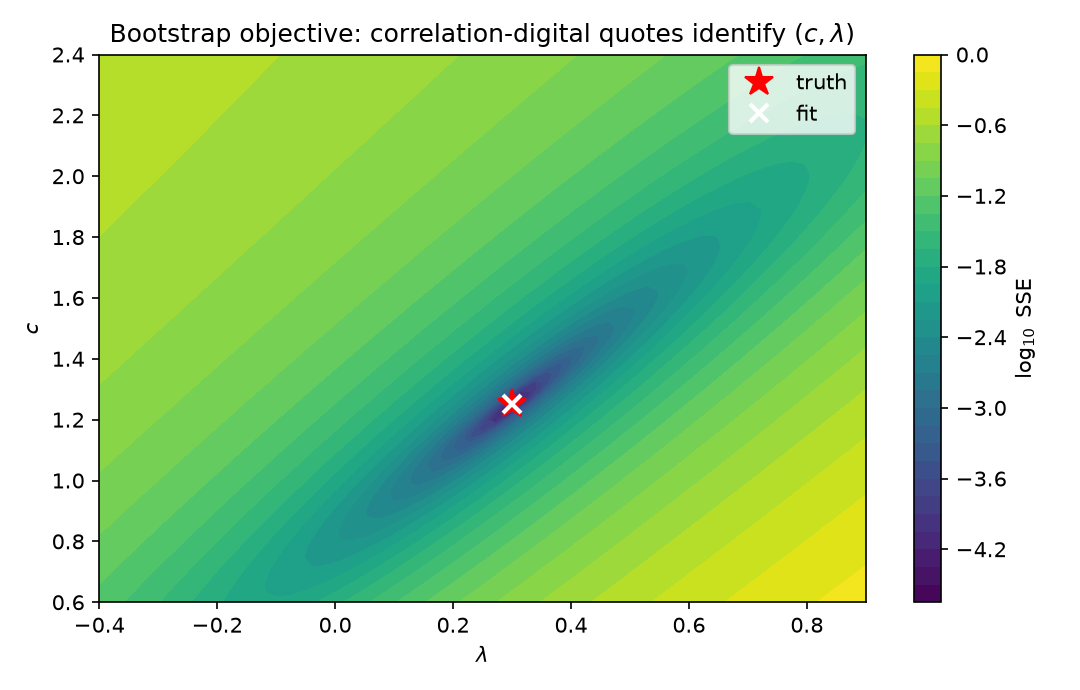
\includegraphics[keepaspectratio]{figures/phase7_bootstrap.png}}

}

\caption{\label{fig-bootstrap}Bootstrap objective landscape in
\((\lambda,c)\): single funnel around the truth (star), fit (cross).}

\end{figure}%

\section{The proportional-drift barrier class}\label{sec-proportional}

\textbf{Theorem (operational-time reduction).} \emph{Suppose
\(\mu(t)=\lambda\sigma^2(t)\) a.e. on \([0,T]\) with \(\sigma(t)>0\).
Then} \[X_t \;\overset{d}{=}\; x_0+\lambda\,v(t)+B_{v(t)}\] \emph{for a
Brownian motion \(B\), and consequently every first-passage,
perpetual-hitting, and band-exit law of the constant-coefficient theory
holds verbatim with calendar time replaced by \(u=v(T)\); e.g.} \[
P(\tau_{\rho^*}\le T)=
\Phi\!\Big(\frac{\lambda u-b}{\sqrt u}\Big)+e^{2\lambda b}
\Phi\!\Big(-\frac{\lambda u+b}{\sqrt u}\Big),
\qquad u=v(T),\quad b=x(\rho^*)-x_0 .
\]

The proof is one line of DDS plus monotonicity of \(v\). Two
consequences deserve emphasis.

\textbf{Parsimony corollary.} Barrier laws depend on \(\sigma(\cdot)\)
only through \(u=v(T)\): rescaling the volatility curve leaves them
bit-identical (verified numerically: identical exact CDFs, both
bridge-corrected Monte Carlo benchmarks within 1 SE). The pair
\((c,\lambda)\) determines all barrier prices; \(\sigma(\cdot)\) merely
warps calendar time.

\textbf{Necessity within the catalog.} Off proportionality,
constant-level hitting becomes curved-boundary crossing in operational
time, for which the classical catalog provides series/integral-equation
methods but no closed forms beyond affine boundaries and isolated
families (Durbin 1992; Pötzelberger and Wang 2001; Kahalé 2008).
Proportionality is therefore the only general deterministic-coefficient
class inheriting the full reflection toolkit; beyond it we state this as
a conjecture relative to the catalog.

\textbf{Calendar-time cost.} Pay-at-hit discounting maps through
\(v^{-1}\): \(E[e^{-r\tau}]\) retains a closed form only when \(v\) is
affine (constant \(\sigma\)). This is the honest price of the reduction.

Verification: hitting CDFs against bridge-corrected exact-skeleton
simulation for humped and oscillating curves agree within
\textasciitilde1 SE at two step sizes ((\textbf{tab-proportional?})).

\begin{longtable}[]{@{}
  >{\raggedright\arraybackslash}p{(\linewidth - 8\tabcolsep) * \real{0.2000}}
  >{\raggedright\arraybackslash}p{(\linewidth - 8\tabcolsep) * \real{0.2000}}
  >{\raggedright\arraybackslash}p{(\linewidth - 8\tabcolsep) * \real{0.2000}}
  >{\raggedright\arraybackslash}p{(\linewidth - 8\tabcolsep) * \real{0.2000}}
  >{\raggedright\arraybackslash}p{(\linewidth - 8\tabcolsep) * \real{0.2000}}@{}}
\caption{Hitting \(\rho^*=0.55\) by \(T=2\) under the proportional
class: identical exact laws for equal integrated
variance.}\label{tbl-proportional}\tabularnewline
\toprule\noalign{}
\begin{minipage}[b]{\linewidth}\raggedright
curve
\end{minipage} & \begin{minipage}[b]{\linewidth}\raggedright
\(u(T)=v(2)\)
\end{minipage} & \begin{minipage}[b]{\linewidth}\raggedright
exact
\end{minipage} & \begin{minipage}[b]{\linewidth}\raggedright
MC(100)
\end{minipage} & \begin{minipage}[b]{\linewidth}\raggedright
MC(400)
\end{minipage} \\
\midrule\noalign{}
\endfirsthead
\toprule\noalign{}
\begin{minipage}[b]{\linewidth}\raggedright
curve
\end{minipage} & \begin{minipage}[b]{\linewidth}\raggedright
\(u(T)=v(2)\)
\end{minipage} & \begin{minipage}[b]{\linewidth}\raggedright
exact
\end{minipage} & \begin{minipage}[b]{\linewidth}\raggedright
MC(100)
\end{minipage} & \begin{minipage}[b]{\linewidth}\raggedright
MC(400)
\end{minipage} \\
\midrule\noalign{}
\endhead
\bottomrule\noalign{}
\endlastfoot
humped & 2.078244 & 0.67685 & 0.67608 (0.00105) & 0.67628 (0.00105) \\
oscillating, rescaled & 2.078244 & 0.67685 & 0.67766 (0.00105) & 0.67605
(0.00105) \\
\end{longtable}

\section{A Feynman--Kac pitfall and the correct
engine}\label{sec-pitfall}

The clock characteristic function \(\phi_A(\xi)=E[e^{i\xi A_T}]\),
\(A_T=\int_0^T f(X_s)\,ds\), was computed in the companion paper by
solving the \textbf{backward} equation

\[
\partial_t u=\tfrac12\sigma^2\partial_{xx}u+\mu\partial_xu+i\xi f(x)u,
\qquad u(0,x)=1,
\]

--- legitimate there because coefficients were constant. For
deterministic curves the naive extension is \textbf{false}.

\textbf{Proposition (counterexample).} \emph{Let \(\sigma\equiv0\),
\(\mu(t)=t\). Then \(X_t=x+t^2/2\) deterministically and}

\[
u(t,x)=e^{i\xi(xt+t^3/6)}
\]

\emph{satisfies \(\partial_tu=i\xi(x+t^2/2)u\) while the backward
equation demands \(\partial_tu=\mu(t)\partial_xu+i\xi xu=i\xi(x+t^2)u\).
These differ whenever \(\mu'(t)\ne0\).}

The root cause: the derivation of the backward equation conditions the
future segment on \(\mathcal F_{dt}\) and replaces
\(E[e^{q\int_{dt}^{t+dt}f}]\) by \(u(t,X_{dt})\) --- valid iff the
propagator is time-translation invariant, i.e.~iff coefficients are
constant.

\textbf{Correct primitive.} The \emph{forward} Feynman--Kac
(Fokker--Planck with potential) equation for the tilted density \(p\),

\[
\partial_tp=\tfrac12\sigma^2(t)p_{xx}-\mu(t)p_x+q(x)p,
\qquad p(0,x)=\delta(x-x_0),
\qquad \phi=\int p(T,x)\,dx ,
\]

is valid unconditionally (it is the forward equation of the tilted
semigroup) and reduces to the familiar object for constant coefficients
--- which retro-explains why the pitfall stayed hidden through six
phases of constant-coefficient work.

Implementation: Crank--Nicolson stepping with midpoint-frozen
coefficients, Dirichlet localization, delta bump as a narrow normalized
Gaussian. Verification ladder ((\textbf{tab-fk?})):

\begin{longtable}[]{@{}
  >{\raggedright\arraybackslash}p{(\linewidth - 2\tabcolsep) * \real{0.5000}}
  >{\raggedright\arraybackslash}p{(\linewidth - 2\tabcolsep) * \real{0.5000}}@{}}
\caption{Verification of the forward-FK solver.
\{\#tab-fk\}}\tabularnewline
\toprule\noalign{}
\begin{minipage}[b]{\linewidth}\raggedright
check
\end{minipage} & \begin{minipage}[b]{\linewidth}\raggedright
result
\end{minipage} \\
\midrule\noalign{}
\endfirsthead
\toprule\noalign{}
\begin{minipage}[b]{\linewidth}\raggedright
check
\end{minipage} & \begin{minipage}[b]{\linewidth}\raggedright
result
\end{minipage} \\
\midrule\noalign{}
\endhead
\bottomrule\noalign{}
\endlastfoot
constant coefficients vs Phase-6 exponential solver (\(\xi=0.7,2.1\)) &
\(2\cdot10^{-4}\) \\
linear potential, variable coefficients vs Gaussian closed form &
\(4.2\cdot10^{-4}\) \\
spatial convergence (grids 900/1800/3600, \(\xi=0.3\)) & 1.69e-3 →
4.22e-4 → 1.05e-4 \\
\(\phi(0)=1\) under variable curves & \(10^{-6}\) \\
margin doubling at fixed \(h\) & \(<10^{-3}\) \\
bounded map vs MC, \(\xi\in\{0.5,1.5,3\}\) & ≤4 SE real \& imag \\
\(E[A_T]\): PDE central difference vs exact marginal quadrature &
\(2\cdot10^{-5}\) \\
\end{longtable}

For contrast, the \emph{incorrect} backward implementation returned
\(\phi(0.5)=0.9060+0.0428j\) against truth \(0.9094+0.0651j\) and
implied \(E[A_T]=0.0892\) against the exact \(0.13454\). The real parts
nearly agree; the damage concentrates in the path-dependent imaginary
structure --- which is why marginal-only validation would have certified
the wrong solver.

\section{Related literature}\label{sec-related}

Static inheritance rests on textbook Gaussianity; our contribution is
its systematic organization into pricing objects for a bounded state,
including the quantile term structure absent from the audited corpus
(Teng--Ehrhardt--Günther and successors calibrate stationary densities;
Wishart multi-curve models approximate). The proportional-drift class is
new as a classification; DDS itself and curved-boundary numerics are
classical (Durbin 1992; Pötzelberger and Wang 2001; Kahalé 2008). The FK
pitfall appears unpublished: standard references state Feynman--Kac for
autonomous generators or handle time-dependence by state-space
augmentation, and the numerical literature on moving-boundary/occupation
problems does not flag the failure mode demonstrated here.

\section{Conclusion}\label{sec-conclusion}

Deterministic coefficient curves split the exact-law program cleanly:
finite-dimensional laws inherit fully; reflection laws survive on the
proportional-drift class and collapse to a clock; and the occupation-
transform engine must be rebuilt on the forward equation. All three
pieces are implemented, unit-tested, and Monte Carlo-verified, providing
the platform on which the companion papers build Fourier pricing (Phase
8), exact estimation (Phase 9), matrix-valued extensions (Phase 10),
Lévy drivers (Phase 11), and pegged-asset economics (Phase 12).

\section{Reproducibility}\label{sec-repro}

Environment: conda \texttt{phase3-paper} (Python 3.12.13, numpy 2.5.1,
scipy 1.18.0, matplotlib 3.11.1). Notebook:
\texttt{notebooks/phase7\_term\_structure.ipynb} (executed clean,
\textasciitilde21 s, seed 20260821); builder
\texttt{notebooks/build\_phase7\_term\_structure.py}; module
\texttt{phase7\_term\_structure.py}; tests
\texttt{tests/test\_phase7\_term\_structure.py} (21/21). Figures
regenerate deterministically from the notebook.

\protect\phantomsection\label{refs}
\begin{CSLReferences}{1}{1}
\bibitem[\citeproctext]{ref-durbin1992}
Durbin, James. 1992. {``The First-Passage Density of a Continuous
Gaussian Process to a General Boundary.''} \emph{Journal of Applied
Probability} 29 (2): 291--304.

\bibitem[\citeproctext]{ref-kahale2008}
Kahalé, Nabil. 2008. {``Analytical Crossing Probabilities for Barriers
with Moving Boundaries.''} \emph{Annals of Applied Probability} 18 (5):
1960--83.

\bibitem[\citeproctext]{ref-potzelberger2001}
Pötzelberger, Klaus, and Lixing Wang. 2001. {``Boundary Crossing
Probability for Brownian Motion.''} \emph{Journal of Applied
Probability} 38 (1): 152--64.

\bibitem[\citeproctext]{ref-teng2016}
Teng, Long, Matthias Ehrhardt, and Michael Günther. 2016. {``Modelling
Stochastic Correlation.''} \emph{Journal of Mathematics in Industry} 6
(1): 1--18. \url{https://doi.org/10.1186/s13362-016-0018-4}.

\end{CSLReferences}




\end{document}
